\documentclass[a4paper,11pt,twocolumn]{article}

\usepackage{aas_macros}

\usepackage[utf8]{inputenc}
\usepackage[T1]{fontenc}
\usepackage{lmodern}
%\usepackage{times}
%\usepackage[margin=2cm]{geometry}
\usepackage[a4paper]{geometry}
\usepackage{amsmath}
\usepackage{mathtools}
\usepackage{graphicx}
\usepackage{multirow}
\usepackage{blindtext}
\usepackage{hyperref}
\usepackage{float}

\usepackage{pgfplotstable}
\usepackage{booktabs}
% \pgfplotsset{compat=1.18}


\graphicspath{ {./images/} }

\usepackage[czech]{babel}
\usepackage{graphicx}
\usepackage{amsmath}
\usepackage{xspace}
\usepackage{url}
\usepackage{siunitx}
\usepackage{indentfirst}
\usepackage{subcaption}
\usepackage{caption}
\usepackage{tabularx}
\usepackage{rotating}
\usepackage{tikz}
\usepackage[labelformat=parens,labelsep=quad,skip=3pt]{caption}

\usepackage{color}
\usepackage{listings}

\definecolor{codegreen}{rgb}{0,0.6,0}
\definecolor{codegray}{rgb}{0.5,0.5,0.5}
\definecolor{codepurple}{rgb}{0.58,0,0.82}
\definecolor{backcolour}{rgb}{0.95,0.95,0.92}

\lstdefinestyle{mystyle}{
    backgroundcolor=\color{backcolour},
    commentstyle=\color{codegreen},
    keywordstyle=\color{magenta},
    numberstyle=\tiny\color{codegray},
    stringstyle=\color{codepurple},
    basicstyle=\ttfamily\footnotesize\centering,
    breaklines=true,
    captionpos=b,
    numbers=left,
    numbersep=5pt,
    showspaces=false,
    showstringspaces=false,
    showtabs=false,
    tabsize=2
}

\lstset{style=mystyle}

%\widowpenalty 10000 \clubpenalty 10000 \displaywidowpenalty 10000
\setcounter{topnumber}{3}
\setcounter{bottomnumber}{3}
\setcounter{totalnumber}{6}
\renewcommand\topfraction{0.9}
\renewcommand\bottomfraction{0.9}
\renewcommand\textfraction{0.1}
\intextsep=8mm \textfloatsep=8mm

\renewcommand{\thesection}{\arabic{section}.}
\renewcommand{\thesubsection}{\thesection\arabic{subsection}.}
\makeatletter \def\@seccntformat#1{\csname the#1\endcsname\hspace{1ex}} \makeatother


\begin{document}
    \twocolumn[
    \noindent\hrulefill
    \begin{center}
        \bigskip
        \huge Pink Floyd
        \vspace{0.2cm}
        \par \large F4191: Praktikum z astronomie 2
        \par \large Artem Gorodilov
        \vspace{0.2cm}
        \par \large 1. ~ledna 2025
        \bigskip
    \end{center}
    \noindent\hrulefill
    \bigskip
    ]

    \vskip10pt
    \section{Abstrakt}
        V této práci jsem vytvořil sRGB obraz loga vynikajícího alba Pink Floyd The Dark Side of the Moon ze snímků pořízených CCD kamerou ve třech BVR filtrech.
        
        Výpočty byly provedeny pomocí skriptu v Pythonu\textsuperscript{\cite{github}}.
    \section{Úvod}
        \subsection{Pink Floyd}
            Pink Floyd je britská rocková skupina, která vznikla v roce 1965. Je známá svými konceptuálními alby a progresivním rockem. Jedním z nejznámějších alb skupiny je The Dark Side of the Moon, které bylo vydáno v roce 1973. Obal alba byl navržen Stormem Thorgersonem a Hipgnosis (viz. obr \ref{fig:pink_floyd}) a je považován za jedno z nejlepších alb všech dob. A s pisničkou Time je to prostě bomba.

            \begin{figure}
                \centering
                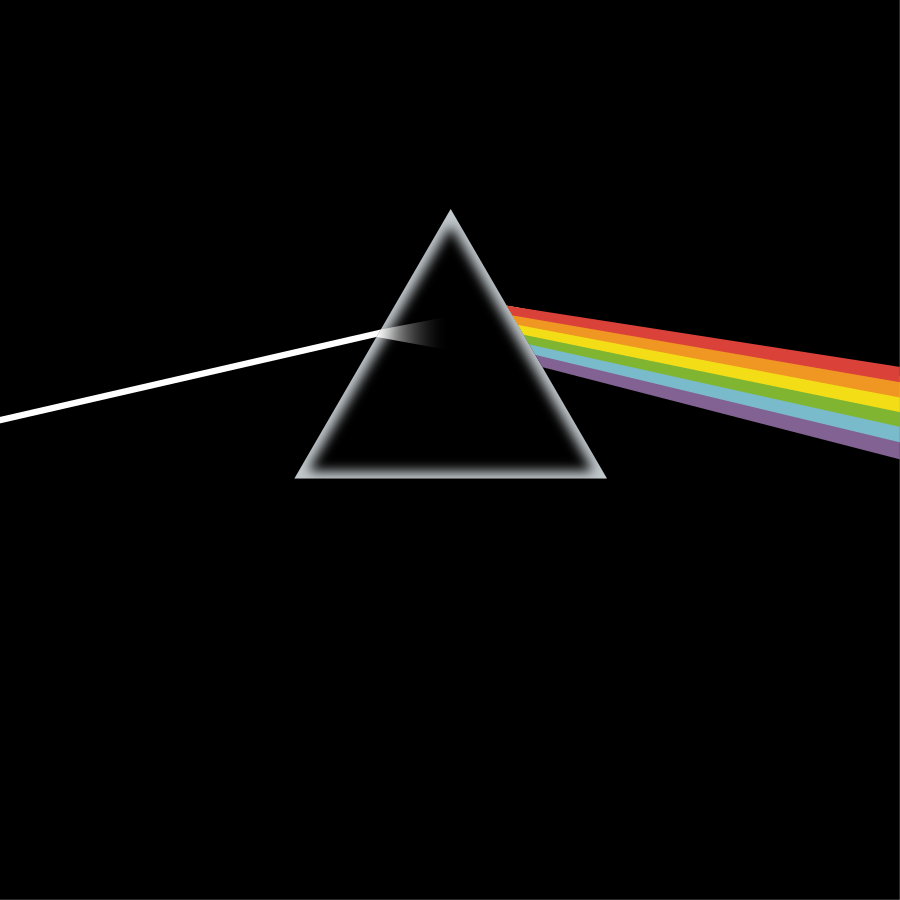
\includegraphics[width=0.5\textwidth]{pf}
                \caption{Obal alba zobrazuje světlo lámající se v trojúhelníkovém disperzním hranolu.}
                \label{fig:pink_floyd}
            \end{figure}
        
        \subsection{Johnson BVR}
            Johnsonův BVR\textsuperscript{\cite{1953ApJ...117..313J}}  systém je fotometrický systém používaný k měření jasnosti hvězd ve třech specifických pásmech: B (blue, modré), V (visual, viditelné) a R (red, červené) (viz. obr \ref{fig:john}). Tyto filtry odpovídají různým částem spektra: modrému světlu (410 nm), zelenému světlu blízkému lidskému vnímání (550 nm) a červenému světlu (700 nm).

            \begin{figure}
                \centering
                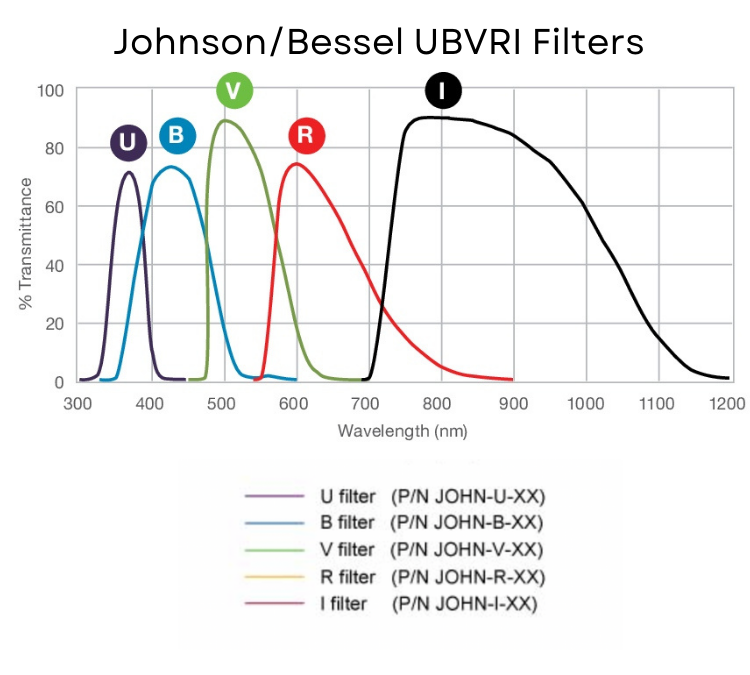
\includegraphics[width=0.5\textwidth]{john}
                \caption{Johnsonův UBVRI systém.}
                \label{fig:john}
            \end{figure}

            Důležitost BVR systému spočívá v jeho schopnosti přesně zaznamenat světlo z astronomických objektů přes různé filtry, což umožňuje rekonstruovat barevné obrázky. Kombinací snímků z jednotlivých filtrů lze vytvořit věrný barevný obraz, který odpovídá skutečnému vzhledu objektů (viz. obr \ref{fig:rgb}). Tento postup nejen poskytuje esteticky působivé snímky, ale také slouží jako cenný nástroj pro studium fyzikálních vlastností hvězd, galaxií a mlhovin, jako jsou jejich teplota, složení a rozložení prachu.

            \begin{figure}
                \centering
                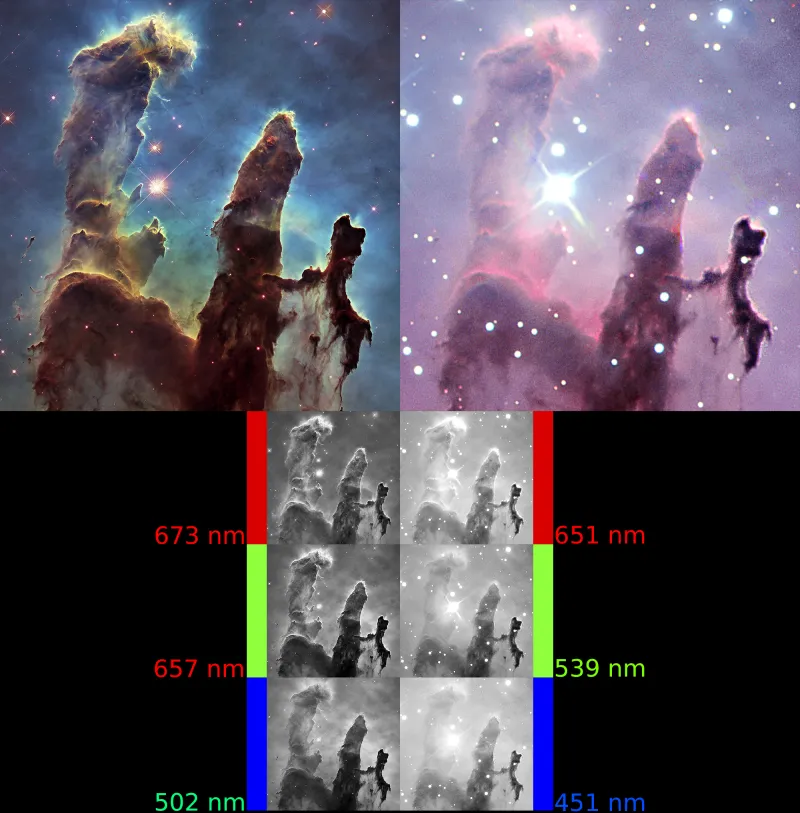
\includegraphics[width=0.5\textwidth]{rgb}
                \caption{“Pillars of Creation” in the Eagle Nebula (M16, NGC 6611). The image on the left was taken by the Hubble Space Telescope, the image on the right by the MPG/ESO 2.2-meter telescope. }
                \label{fig:rgb}
            \end{figure}

        \subsection{CIE 1931}
            CIE 1931\textsuperscript{\cite{1931TrOS...33...73S}} barevný systém je jedním z prvních matematických modelů pro popis lidského vnímání barev. Založen je na třech primárních barvách (X, Y, Z), které nejsou skutečnými barvami, ale matematickými konstrukcemi. Hodnota Y odpovídá jasu (luminance), zatímco X a Z reprezentují barevné informace (chromaticity). Barevný prostor CIE 1931 zahrnuje všechny barvy, které průměrný člověk dokáže vidět, a je často zobrazován jako diagram barevného trojúhelníku (viz. obr \ref{fig:cie}).

            \begin{figure}
                \centering
                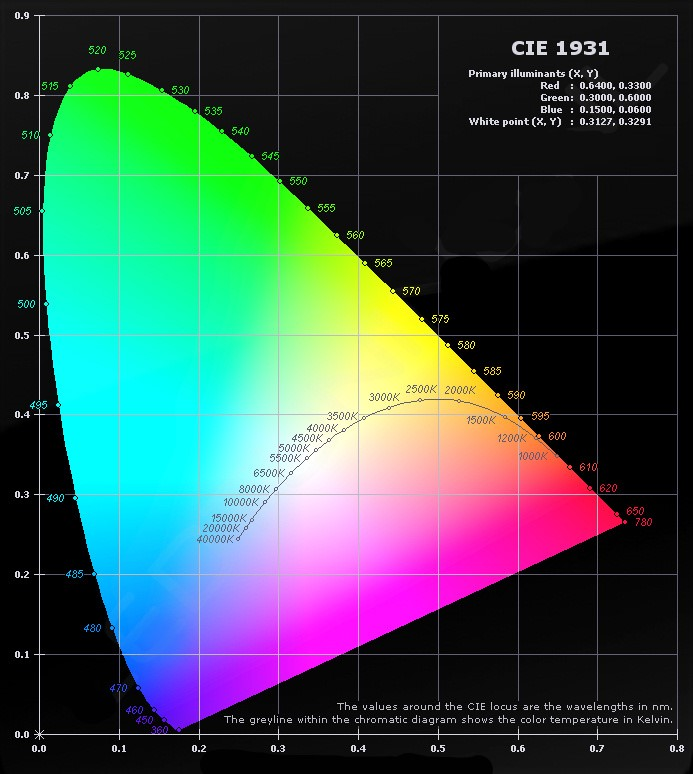
\includegraphics[width=0.5\textwidth]{cie}
                \caption{CIE 1931 barevný prostor.}
                \label{fig:cie}
            \end{figure}

            Pro převod z BVR (fotometrický systém) do CIE XYZ používáme transformaci definovanou maticí, která závisí na transmisních vlastnostech filtrů B, V, R a spektrální citlivosti systému XYZ:

            \begin{equation}
                \begin{bmatrix}
                    X \\
                    Y \\
                    Z
                \end{bmatrix}
                =
                \begin{bmatrix}
                    0.19362 & 0.59315 & 0.31060 \\
                    0.08265 & 1.10069 & 0.08009 \\
                    1.38826 & -0.11459 & 0.01970
                \end{bmatrix}
                \begin{bmatrix}
                    B \\
                    V \\
                    R
                \end{bmatrix}
                \label{brv_xyz}
            \end{equation}

            Hodnoty matice jsou experimentálně určeny a liší se podle použitých filtrů.

            CIE XYZ je standardní model a pro převod do RGB barevného prostoru (např. sRGB) se opět používá transformační matice. Pro sRGB prostor je matice následující:

            \begin{equation}
                \begin{bmatrix}
                    R \\
                    G \\
                    B
                \end{bmatrix}
                =
                \begin{bmatrix}
                    3.2410 & -1.5374 & -0.4986 \\
                    -0.9692 & 1.8760 & 0.0416 \\
                    0.0556 & -0.2040 & 1.0570
                \end{bmatrix}
                \begin{bmatrix}
                    X \\
                    Y \\
                    Z
                \end{bmatrix}
                \label{xyz_rgb}
            \end{equation}

            Výsledné hodnoty $R, G, B$ mohou být mimo rozsah [0, 1], a je potřeba je oříznout na tento interval.

            Pro zobrazení na monitorech (které mají nelineární odezvu) je nutné aplikovat gamma korekci. Pro sRGB standard je gamma korekce definována takto:

            \begin{equation}
                g(x) =
                \begin{cases} 
                    12.92x, & x \leq \tau, \\
                    1.055x^{1/2.4}-0.055, & x > \tau.
                \end{cases}
                \label{gamma}
            \end{equation}
            
            kde $\tau = 0.0031308$.

            Tento proces se aplikuje na všechny kanály $g(R), g(G), g(B)$.  Výsledkem je obraz optimalizovaný pro lidské vnímání na digitálních zobrazovacích zařízeních.
        
    \section{Zpracování dat}
        Ke složení barevného obrazu sRGB jsem použil snímky plakátu PF TDSotM pořízené CCD kamerou ve třech filtrech $B, V, R$. Všechny snímky měly expozici 1 s. Pro kvalitativní analýzu jsem vybral pouze oblast snímku, kde se nachází plakát. Použité snímky, názvy souborů a jim odpovídající filtry jsou uvedeny na obrázku (\ref{fig:pf_ind}).

        \begin{figure}
            \centering
            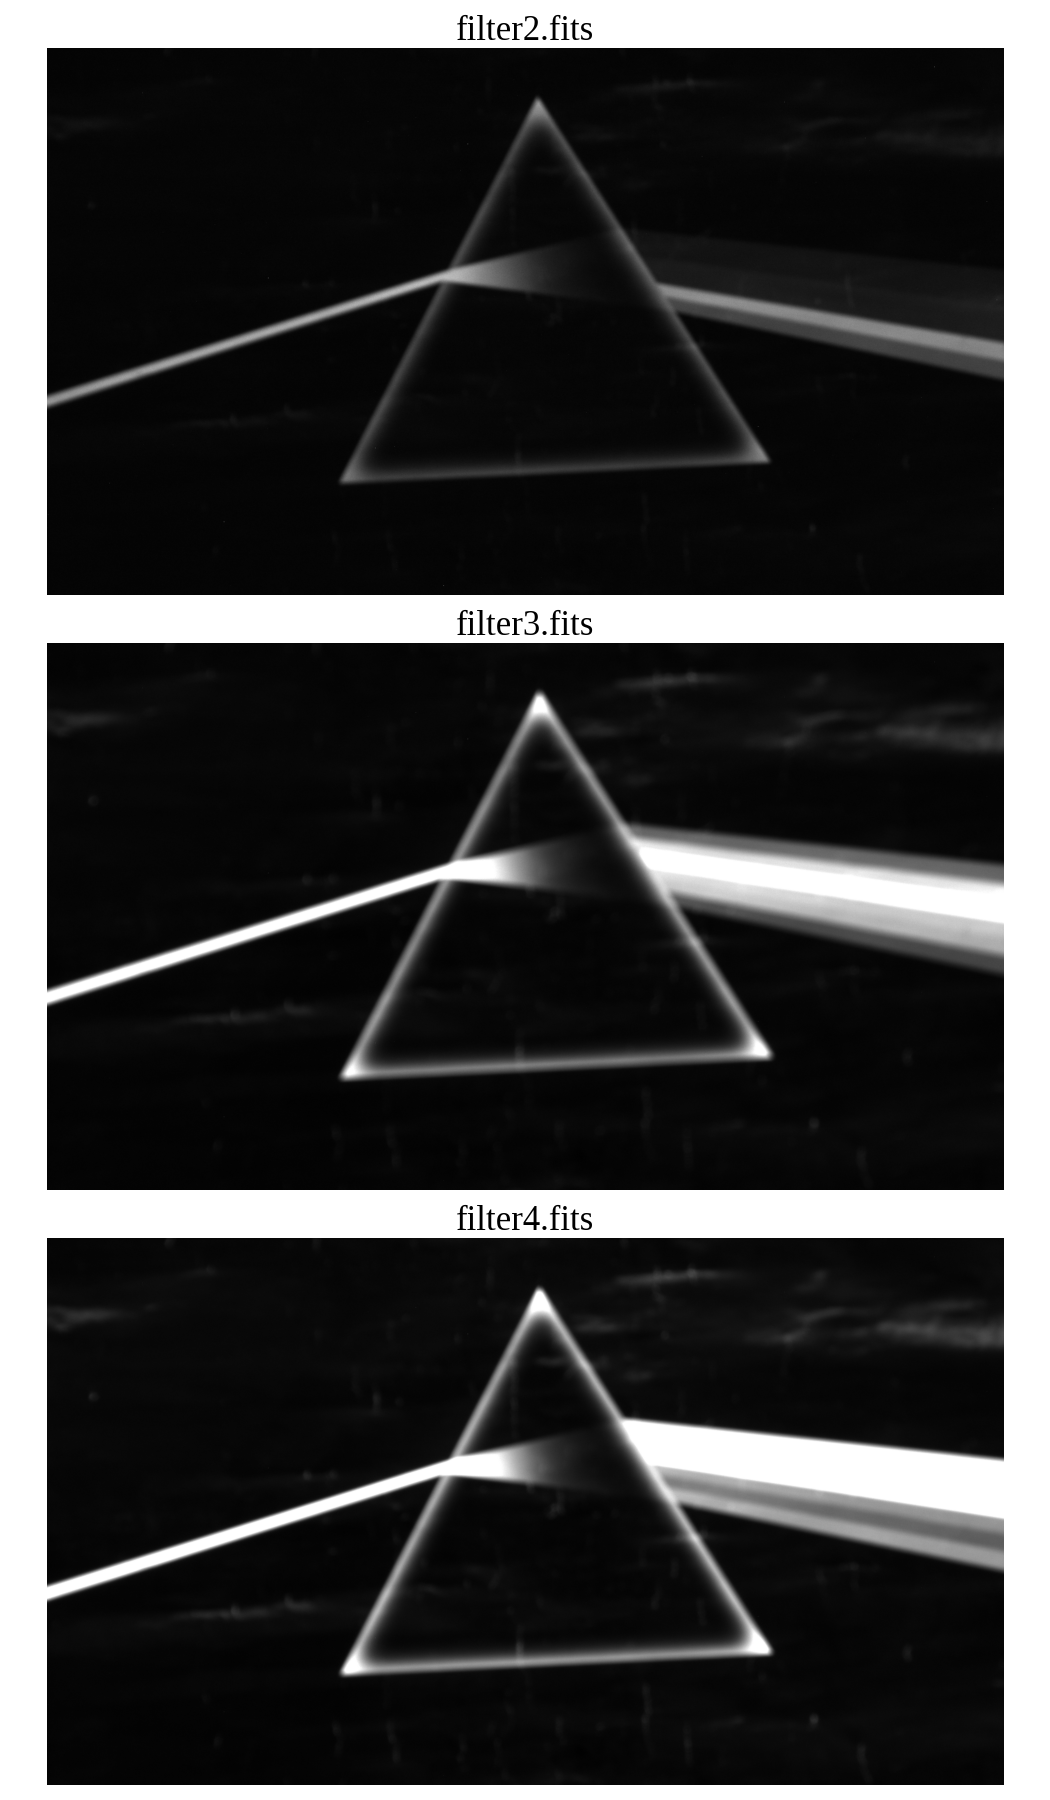
\includegraphics[width=0.5\textwidth]{pf_ind}
            \caption{Snímky plakátu PF TDSotM pořízené ve filtrech B, V, R (zhora dolů).}
            \label{fig:pf_ind}
        \end{figure}
        
        Poté jsem vybral oblast pozadí snímku, zjistil medián intenzity pro každý snímek a provedl jeho odečtení. Oblast pozadí je vidět na obrázku (\ref{fig:pf_srgb}). Poté jsem normalizoval BVR snímku tak, aby intenzity jednotlivých pixelů byly v rozmezí [0,1]. K tomuto účelu jsem použil vzorec:  

        \begin{equation}
            I_{\text{norm}} = \frac{I - I_{\text{min}}}{I_{\text{max}} - I_{\text{min}}}
        \end{equation}

        kde $I_{\text{min}}$ a $I_{\text{max}}$ jsou minimální a maximální intenzity pixelů v oblasti pozadí.

        Poté jsem převedl snímky BVR na XYZ pomocí vzorce (\ref{brv_xyz}).  Poté jsem získané hodnoty také normalizoval. 
        
        Potom bylo nutné vyvážit bílou barvu. Pro tento účel jsem vybral snímek na snímku Y, kde světlo vstupuje do hranolu a má bílou barvu. Vybranou oblast můžete vidět na obrázku (\ref{fig:pf_srgb}). Zjistil jsem medián intenzity $I_{\text{Y}}$ v této oblasti a poté jsem podle vzorců vypočítal škálovací koeficienty pro obrazy X a Z: 

        \begin{equation}
                k_{\text{X}} = 0.9505 \frac{I_{\text{Y}}}{I_{\text{X}}}, ~~
                k_{\text{Z}} = 1.0890 \frac{I_{\text{Y}}}{I_{\text{Z}}}
        \end{equation}

        Z toho jsem upravil hodnoty intenzity jednotlivých snímků: 

        \begin{equation}
            I_{\text{X}} = k_{\text{X}} I_{\text{X}}, ~~
            I_{\text{Z}} = k_{\text{Z}} I_{\text{Z}}
        \end{equation}

        Poté jsem převedl obrázky XYZ na RGB pomocí vzorce (\ref{xyz_rgb}). Před použitím funkce Gamma jsem se ujistil, že hodnoty intenzity v obrázcích RGB budou v hodnotách [0,1]. K tomuto účelu jsem použil funkci \texttt{np.clip(rgb\_images, 0, 1)}, která se často používá pro Gamma korekce. Gama korekci jsem provedl podle vzorce (\ref{gamma}).

    \section{Vysledky}
        Výsledné sRGB, BVR a XYZ obrazy plakátu PF TDSotM jsou zobrazeny na obrázcích (\ref{fig:pf_srgb}), (\ref{fig:pf_bvr}) a (\ref{fig:pf_xyz}).
        
        \begin{figure}
            \centering
            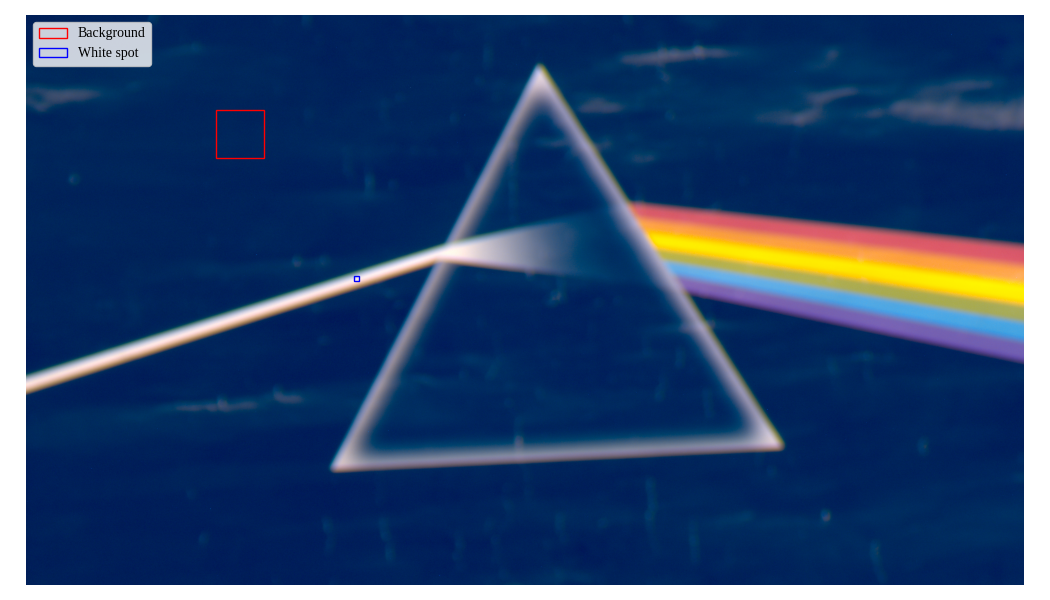
\includegraphics[width=0.5\textwidth]{pf_srgb}
            \caption{Výsledný sRGB obraz plakátu PF TDSotM.}
            \label{fig:pf_srgb}
        \end{figure}

        \begin{figure}
            \centering
            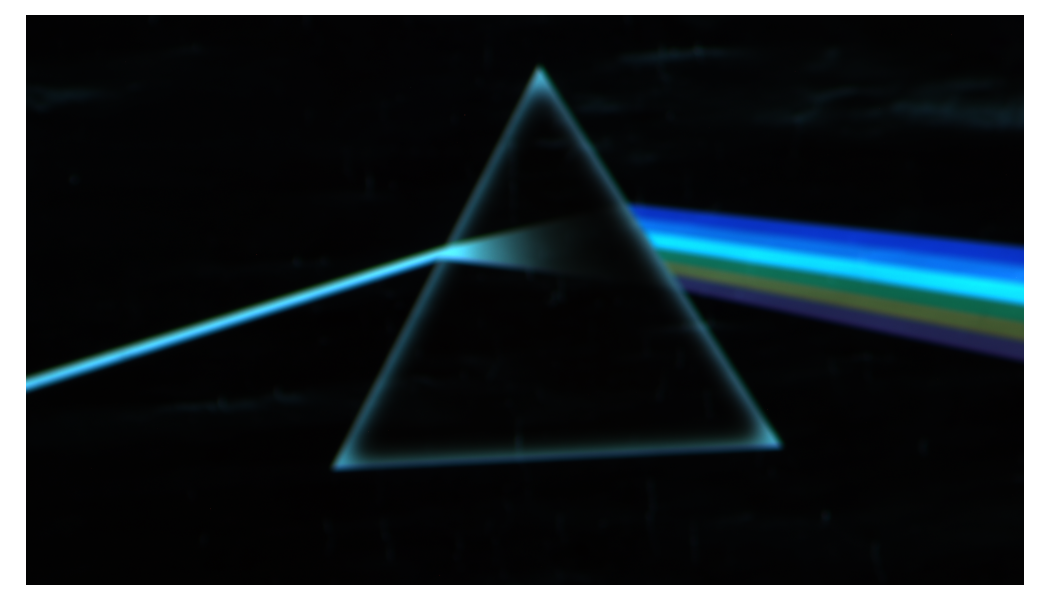
\includegraphics[width=0.5\textwidth]{pf_bvr}
            \caption{Výsledný BVR obraz plakátu PF TDSotM (pozadí odečteno).}
            \label{fig:pf_bvr}
        \end{figure}

        \begin{figure}
            \centering
            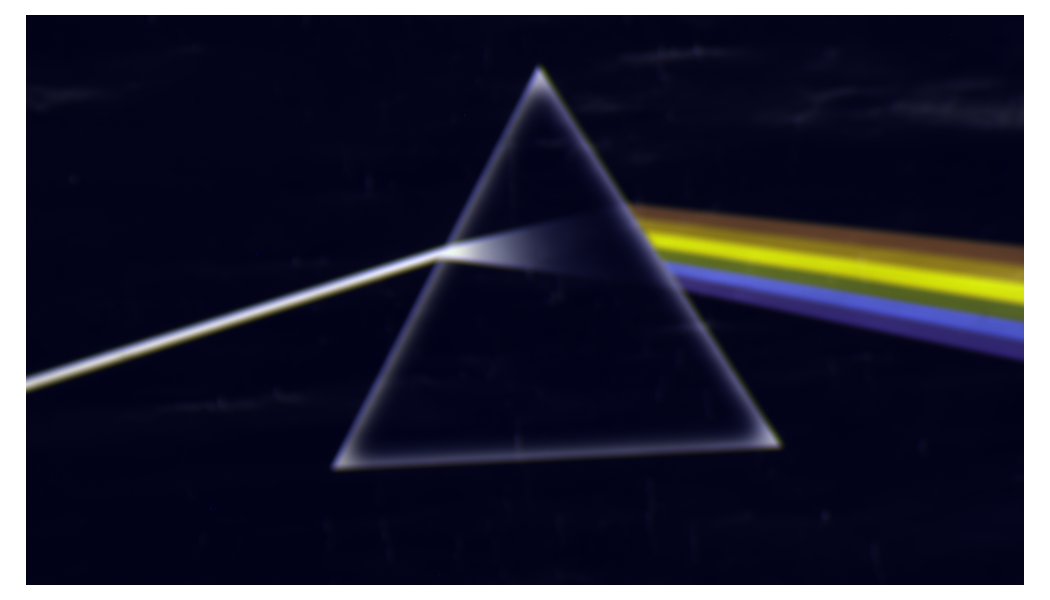
\includegraphics[width=0.5\textwidth]{pf_xyz}
            \caption{Výsledný XYZ obraz plakátu PF TDSotM.}
            \label{fig:pf_xyz}
        \end{figure}

    \section{Závěr}
        Výsledné sRGB obrazy jsou věrnými reprezentacemi barev plakátu a zachovávají jeho estetickou hodnotu. Jako reference je uveden obrázek plakátu (\ref{fig:original}) pořízený zrcadlovkou.  Zásadní rozdíl je v pozadí. Na rozdíl od původní barvy plakátu (černá) má pozadí tmavě modrý nádech. Domnívám se, že by to mohlo být způsobeno tím, že světlo, které bylo v tu chvíli v místnosti, mělo teplotu $2700-3000$ K a mělo teplou žlutou barvu. Potvrzuje to i vysoká intenzita žluté čáry v prizmatem rozloženém spektru ve $V$ a $R$ filtru. 
        
        Barevné rozdíly mezi snímky jsou způsobeny různými transmisemi filtrů BVR a spektrální citlivostí lidského oka. Výsledné XYZ obrazy jsou věrnými reprezentacemi barev plakátu v CIE 1931 barevném prostoru. BVR obrazy ukazují intenzitu světla v jednotlivých pásmech a umožňují studium spektrálních vlastností plakátu.

        \begin{figure}
            \centering
            \includegraphics[width=0.5\textwidth]{IMG_1124.png}
            \caption{Původní snímek plakátu PF TDSotM pomoci zrcadlovky.}
            \label{fig:original}
        \end{figure}
    
    \newpage
    \bibliographystyle{plain}
    \nocite{*}
    \bibliography{refs/github, refs/john, refs/cie}
\end{document}